\documentclass[11pt]{article}
% ACL-style preprint build of docs/paper-apc-en.md — DO NOT EDIT; run paper/build.py.
% Mechanical conversion: inline arXiv-ID citations stay as text; camera-ready switches to .bib+natbib.
\usepackage[final]{acl}
\usepackage{times,latexsym,amsmath,amssymb}
\usepackage{booktabs,longtable,array,multirow,calc}
\usepackage{graphicx,microtype,url,xcolor,textcomp}
\usepackage{tikz}
\usetikzlibrary{positioning}
\setcounter{secnumdepth}{0} % md headings carry their own 3.4m-style numbers
\sloppy
\providecommand{\tightlist}{\setlength{\itemsep}{0pt}\setlength{\parskip}{0pt}}
\title{Adaptive Prompt Compiler: A Headroom Typology for Prompt Optimization\\ on Real Reasoning Models (Anonymous Preprint v0.3)}
\author{Anonymous submission}
\begin{document}
\maketitle
\begin{abstract}
APC turns prompts from hand-written text into compilable engineering objects: a task specification (TaskSpec) compiles, together with an explicit 15-dimensional model profile (ModelProfile), through a discrete 10-gene genome (PromptGenome) into a prompt, which is then improved by budget-aware evolutionary search (with a profile-guided mutation operator, PGAM) and carried across models by structural migration. On a deterministic four-task benchmark (APCBench; financial/contract/math/constraint-following \(\times\) 3 simulated model profiles): search significantly beats zero-shot (+0.009 to +0.029); evolution beats random search on compositional tasks (+0.003) but loses on single-locus tasks (-0.013, successive-halving selection noise); PGAM is indistinguishable from uniform mutation (pooled +0.0004, a null result; its first real-model test, gpt-6 math, runs -.0376 vs uniform); migration reaches native-quality at 30\% of the re-search budget (KR-6 passed 12/12). On a real frontier reasoning model (qwen3.8-flash, four arms \(\times\) three tasks, identical rule-judge): accuracy gains of genome search are \(\approx\)0 --- the base-root arm holds the zero-shot floor on all three tasks (within -0.004) while the profile-rule root is a net liability (dev-score deficits of 0.2--0.53, recovered only partially within budget); the strongest deployment policy is \emph{zero-adaptation transfer} of a cross-task champion genome (0 budget, \(\geq\) same-task zero-shot, up to +0.79 over cold re-search). External author-unseen benchmarks (GSM8K, MATH Level-5, AIME 2024+25) reproduce both findings: all six champion-vs-base deltas are within noise and the model saturates every benchmark (AIME: 60/60), bounding the room for prompt optimization on strong reasoners. We distill these into a methodological principle, \emph{Compile-as-Hypothesis}: compiled artifacts are testable hypotheses, never default deployables, and prior value is a measured quantity that can be negative. The multi-model replication matrix (\textbackslash S\{\}3.4p) confirms the task-regime taxonomy for structured genome search and cross-task warm-start migration on two additional frontier reasoning models (gpt-6, gpt-5.6-terra via an OpenAI-compatible gateway), with the seed-42 champion genome byte-identical across all three models --- and surfaces one genuine cross-model divergence: on gpt-6, free-text reflective optimization (GEPA) finds +.14 on financial where genome search has none, a gain we decompose into a quantified judge-gaming component (\textasciitilde.035) and genuine task-instruction improvement (\textasciitilde.105). On the same real API we then close the baseline and regime questions: the official GEPA baseline (Algorithm 1 reproduced) is also within the paired same-day noise band (+.0024), the second strong baseline ESPO likewise (.7009), and a pre-registered token-starved discriminative experiment (F10) pins six pathways at the judge floor (.1500) when headroom is physically unreachable. F11 completes the map on a stratified 90-problem HLE-exact subset --- the first REAL reachable knowledge-type headroom (zero-shot accuracy .10): all six arms tie again (.388-.412); a confirmatory n=100 round replicates the tie (gepa vs z0 McNemar p=.219) and measures the same-text nondeterminism floor at 2.7\%, a GPQA-Diamond round (n=190) replicates the tie on a second real dataset (five arms .853-.868; reflective search accepts zero candidates), even though GEPA demonstrably learned domain content rules (SMILES conventions, perturbation-theory regime qualifiers). The discriminator for prompt-optimization payoff is not whether headroom exists but what kind: physical-truncation and knowledge-type headroom are out of reach for any prompt pathway (ability lives in weights), while protocol/format headroom is reachable and favors structured genomes --- deployment should begin with a headroom-type diagnostic (\textbackslash S\{\}3.4m). A deployment gate (AutoAPC-Select, F8: val-argmax + noise-band Occam tie-break, 5/7 exact-oracle on 7 replay+blind groups) turns these findings into a selection rule. Multi-model validation of PGAM awaits additional API credentials.
\end{abstract}
\subsection{1. Problem and Claim}\label{1-problem-and-claim}

The same business task requires different prompts on different LLMs (Sclar et al. 2023: format sensitivity is model-specific; FLASK, Ye et al. 2024: skill profiles differ per model). Existing evaluation suites (HELM/FLASK) rank models but do not guide prompt construction; existing prompt compilers (DSPy) re-search per model but keep the profile implicit and uninterpretable (see \texttt{docs/\allowbreak{}literature/\allowbreak{}lit-compiler.md} G1--G6).

APC\textquotesingle s claim: \textbf{an explicit capability profile (15 dims) as a compiler intermediate representation} --- \texttt{TaskSpec\ \$\textbackslash{}rightarrow\$\ PromptGenome\ (10\ genes)\ \$\textbackslash{}rightarrow\$\ ModelProfile\ \$\textbackslash{}rightarrow\$\ PromptCompiler\ (rule\ compilation)\ \$\textbackslash{}rightarrow\$\ TrialResult\ \$\textbackslash{}rightarrow\$\ evolutionary\ search\ (PGAM)\ \$\textbackslash{}rightarrow\$\ model\ migration}, fully traceable end-to-end (KR-3).

\textbf{Contributions} (ordered by reviewer concern, not chronology):

\begin{itemize}
\tightlist
\item
  \textbf{C1 \(\cdot\) Profile-driven traceable compilation}: the TaskSpec\(\times\)PromptGenome\(\times\)ModelProfile IR attributes every prompt change to a gene locus and a profile dimension (\textbackslash S\{\}2.1-2.3, F4 decision-chain audit) --- a capability DSPy-style implicit profiles cannot offer.
\item
  \textbf{C2 \(\cdot\) Quantified liability of priors}: the rule-root costs -.090 on a real model (robust across three seeds, including a bimodal seed-collapse case); "compilation priors can be negative and are measurable" --- Compile-as-Hypothesis becomes a quantity, not a slogan (\textbackslash S\{\}3.4 F2/F7).
\item
  \textbf{C3 \(\cdot\) A complete discriminator for APO payoff}: four independent pathways tie in the saturated regime (F7-F9) \(\rightarrow\) all tie under physical truncation (F10) \(\rightarrow\) all tie under reachable knowledge-type headroom, with mechanism evidence that reflection learned content rules yet transferred zero (F11) \(\rightarrow\) while structured pathways win +0.05 in simulated protocol-type headroom. Merged into a \textbf{headroom taxonomy}: when no APO can win --- prior to "whose representation is better" (\textbackslash S\{\}3.4 F10/\textbackslash S\{\}3.4m).
\item
  \textbf{C4 \(\cdot\) Zero-cost deployment gate}: AutoAPC-Select spends measured same-day drift bands as its tie-break currency; on 7 replay+blind groups, 5/7 exact-oracle, both seed-collapse arms rescued at zero regret (\textbackslash S\{\}3.4 F8).
\item
  \textbf{C5 \(\cdot\) Evaluation-methodology assets}: the hardened exact-match judge v3.2 (F6), the paired same-day re-measurement protocol (F7), two empirical instances of the val/holdout common-pool clause (F10/F11), and the connection-layer reliability triad for long-run harnesses (F11) --- all in-repo.
\end{itemize}

\subsection{2. Method}\label{2-method}

\subsubsection{2.1 PromptGenome: a discrete structural genome}\label{21-promptgenome-a-discrete-structural-genome}

Ten gene classes (role/goal/instructions/constraints/examples/reasoning/ verification/output/style/layout); \texttt{search\_\allowbreak{}space} declares mutable loci (13 in our experiments). Unlike continuous soft prompts (Lester 2021; SPoT), a discrete genome is re-compilable and portable across models (\textbackslash S\{\}3.3).

\subsubsection{2.2 Profile-Guided Adaptive Mutation (PGAM)}\label{22-profile-guided-adaptive-mutation-pgam}

\begin{itemize}
\tightlist
\item
  Prior: \texttt{w\ =\ 1\ +\ 2(1\ -\ capability)} truncated to {[}0.5, 3.0{]}; unmapped loci get weight 1.0.
\item
  Online correction: per-generation surviving elite mutation loci \(\times\)1.3 (cap 5.0), floor 0.3 --- an \(\epsilon\)-guarantee that lets the bandit override a mis-specified profile.
\item
  The sole difference from uniform mutation is the locus sampling distribution; scheduling, budget accounting and lineage logging are identical, making the ablation a clean single-variable contrast.
\end{itemize}

\subsubsection{2.3 Budget-aware population + Successive Halving (SHA)}\label{23-budget-aware-population--successive-halving-sha}

\texttt{P\ =\ min(P0,\ max(E+1,\ (B-3)/\allowbreak{}(G+2)))}; per generation dev\_r1 halves the field and dev\_full re-scores. Dev selects, validation names the champion, holdout runs the champion exactly once (the EvoPrompt discipline).

\subsubsection{2.4 Migration protocol (FR-7)}\label{24-migration-protocol-fr-7}

\texttt{CapabilityDelta\ (15\ dims)\ \$\textbackslash{}rightarrow\$\ MigrationMutator\ adjusts\ the\ seed\ \$\textbackslash{}rightarrow\$\ small-budget\ re-search\ on\ target\ \$\textbackslash{}rightarrow\$\ adopt\ iff\ holdout\ \$\textbackslash{}geq\$\ 90\%\ of\ source\ (KR-6)}.

\subsubsection{2.5 Design principle: Compile-as-Hypothesis}\label{25-design-principle-compile-as-hypothesis}

Real-model evidence (\textbackslash S\{\}3.4 F2) forces the principle: \textbf{the output of profile-rule compilation is a hypothesis to be tested, not a deployable default}. The pipeline therefore always runs two roots in parallel at equal budget --- rule-root (apc-full) and base-root (apc-safe) --- and deploys the winner. This makes the implicit assumption of DSPy-style per-model re-search explicit and measurable: prior value = \(\Delta\)(rule-root, base-root), and it can be negative (measured here: 2 of 3 tasks \(\leq\) +0.001; independently corroborated by the capability-dependent compilation gains of arXiv 2608.02639). The principle does not arrive \emph{ex nihilo}: the spirit of deterministic acceptance layers over free-form judging is now established in production-systems literature (PROCTOR catalogues 11 evaluation- signal failure modes with a judge-overridable-proof acceptance gate, arXiv 2609.02246; accept-or-revert gate family: TARA arXiv 2607.18724, arXiv 2606.30840, SSO arXiv 2607.28777; a measurable-prior Bayesian cousin: Textual Bayes arXiv 2506.10060). Our contribution is to \emph{name and operationalize} this practice as a compiler design principle --- both roots permanently in the pipeline --- and to attach quantitative deficit readings (F2/F7). The same principle governs migration: seeds must pass the holdout test before being carried (KR-6).

\subsection{\texorpdfstring{3. Experiments (APCBench, \texttt{experiments/\allowbreak{}apcbench/\allowbreak{}})}{3. Experiments (APCBench, experiments/apcbench/)}}\label{3-experiments-apcbench-experimentsapcbench}

\begin{quote}
\begin{itemize}
\tightlist
\item
  Task A "Financial Report Analysis" (dev 40 / validation 30 / holdout 30 / perturbation 30); Task B "Contract Information Extraction", Task C "Math Word Problems", and Task D "Verifiable Constraint Following" (all dev 40 / validation 30 / holdout 30; generators and seeds are in the respective task scripts). B/C share the \texttt{\_\allowbreak{}prompt\_\allowbreak{}skill} gene dynamics (different domain logic); D uses in-task dynamics (three channels: constraints / sentence count / numbers, activating the instructions/constraints loci that were neutral until now). Perturbation design (A only): distractor sentences + replacement of the first metric value (the gold standard is kept on the clean version).
\item
  Models: glm / qwen / gpt (deterministic simulation via MockClient; ground truth in the README).
\item
  Methods: zero-shot / manual / random-search / apc-full (uniform evolution + SHA) / apc-no-profile / apc-no-halving / apc-pgam.
\item
  Statistics: Task A 5 seeds \(\times\) 3 models, B/C/D 3 seeds \(\times\) 3 models; paired bootstrap 95\% CI.
\end{itemize}
\end{quote}

\subsubsection{3.1 Main results (b100, holdout)}\label{31-main-results-b100-holdout}

{\small
\noindent\begin{tabular}{@{}>{\raggedright\arraybackslash}p{(\linewidth - 8\tabcolsep) * \real{0.25}}>{\raggedright\arraybackslash}p{(\linewidth - 8\tabcolsep) * \real{0.25}}>{\raggedright\arraybackslash}p{(\linewidth - 8\tabcolsep) * \real{0.25}}>{\raggedright\arraybackslash}p{(\linewidth - 8\tabcolsep) * \real{0.25}}@{}}
\toprule
Comparison & \(\Delta\) & 95\% CI & Conclusion \\
\midrule
apc-full - zero-shot & +0.0093 & {[}0.0082, 0.0103{]} & significant; search works \\
apc-pgam - zero-shot & +0.0101 & {[}0.0095, 0.0107{]} & significant \\
evolution - random & +0.0030 & {[}0.0022, 0.0038{]} & significant; value of multi-step composition \\
apc-pgam - apc-full & +0.0008 & {[}0.0000, 0.0017{]} & \textbf{marginal}; variance 0.0001 vs 0.0016 \\
apc-full - manual & -0.0009 & {[}-0.0017, -0.0001{]} & a strong manual heuristic still leads \\
SHA / rules ablation & 0.0000 & --- & null result (base already satisfies the rules) \\
\bottomrule
\end{tabular}}


\subsubsection{3.2 Budget curves (holdout mean)}\label{32-budget-curves-holdout-mean}

\begin{table*}[t]
\centering
\resizebox{0.96\textwidth}{!}{
\begin{tabular}{@{}llllll@{}}
\toprule
budget & pgam & full & random & manual & zero-shot \\
\midrule
25 & 0.7501 & 0.7495 & 0.7497 & 0.7595 & 0.7493 \\
50 & 0.7581 & 0.7581 & 0.7581 & 0.7595 & 0.7493 \\
100 & 0.7600 & 0.7592 & 0.7561 & 0.7600 & 0.7499 \\
\bottomrule
\end{tabular}}
\end{table*}


The plateau is reached at 50 evaluations (a consequence of the task\textquotesingle s unimodality); random in fact degrades at b100 (single-step space + more candidates \(\rightarrow\) dev overfitting).

\subsubsection{3.2b Second task: contract extraction (b50, holdout, n=9/method)}\label{32b-second-task-contract-extraction-b50-holdout-n9method}

\begin{table*}[t]
\centering
\resizebox{0.96\textwidth}{!}{
\begin{tabular}{@{}lllll@{}}
\toprule
Method & Mean & Comparison & \(\Delta\) & 95\% CI \\
\midrule
apc-full / apc-pgam & 0.9844 & search - zero-shot & +0.0275 & {[}0.0130, 0.0420{]}, significant \\
manual & 0.9814 & search - manual & +0.0031 & {[}0.0000, 0.0061{]}, not significant \\
zero-shot & 0.9569 & (qwen alone 0.9300 \(\rightarrow\) search repairs it to 0.9833; weak-model rescue +0.05) & & \\
\bottomrule
\end{tabular}}
\end{table*}


\subsubsection{3.2c Third task: math word problems (b50, holdout, n=9/method)}\label{32c-third-task-math-word-problems-b50-holdout-n9method}

{\small
\noindent\begin{tabular}{@{}>{\raggedright\arraybackslash}p{(\linewidth - 8\tabcolsep) * \real{0.25}}>{\raggedright\arraybackslash}p{(\linewidth - 8\tabcolsep) * \real{0.25}}>{\raggedright\arraybackslash}p{(\linewidth - 8\tabcolsep) * \real{0.25}}>{\raggedright\arraybackslash}p{(\linewidth - 8\tabcolsep) * \real{0.25}}@{}}
\toprule
Comparison & \(\Delta\) & 95\% CI & Conclusion \\
\midrule
search - zero-shot & +0.0285 & {[}0.0191, 0.0372{]} & significant \\
search - manual & -0.0109 & {[}-0.0154, -0.0063{]} & significant; manual is strong (exact count/strategy is hand-optimal) \\
pgam - full & 0.0000 & --- & no difference \\
\bottomrule
\end{tabular}}


Cross-task consistency: search \(\gg\) zero-shot holds on all four tasks (+0.009 / +0.028 / +0.029 / +0.029); search vs manual: financial -0.001, contract +0.003 (n.s.), math -0.011, constraint following +0.024 (significant) --- strong handcrafted heuristics are hard to beat on a unimodal simulator; the value of automation lies in no handwork, plus transfer, plus lineage.

\subsubsection{3.2d Fourth task: verifiable constraint following (b50, holdout, n=9/method)}\label{32d-fourth-task-verifiable-constraint-following-b50-holdout-n9method}

{\small
\noindent\begin{tabular}{@{}>{\raggedright\arraybackslash}p{(\linewidth - 8\tabcolsep) * \real{0.25}}>{\raggedright\arraybackslash}p{(\linewidth - 8\tabcolsep) * \real{0.25}}>{\raggedright\arraybackslash}p{(\linewidth - 8\tabcolsep) * \real{0.25}}>{\raggedright\arraybackslash}p{(\linewidth - 8\tabcolsep) * \real{0.25}}@{}}
\toprule
Comparison & \(\Delta\) & 95\% CI & Conclusion \\
\midrule
search - zero-shot & +0.0292 & {[}0.0171, 0.0399{]} & significant \\
search - manual & +0.0238 & {[}0.0116, 0.0341{]} & significant; search beats manual significantly for the first time \\
random - evolution & +0.0132 & {[}0.0035, 0.0246{]} & significant; direction reversed (see below) \\
pgam - full & +0.0005 & {[}-0.0148, 0.0162{]} & not significant \\
\bottomrule
\end{tabular}}


\textbf{Optimizer cross-decomposition} (after adding a no-halving control for Task D): no-halving (0.9616) \textgreater{} random (0.9513) \textgreater{} SHA evolution (0.938). no-halving - random: +0.0103 {[}0.0022, 0.0205{]} (significant) --- when selection is accurate, the compositional value of multi-step evolution is positive; full - no-halving: -0.0235 {[}-0.0357, -0.0112{]} (significant) --- SHA\textquotesingle s small-sample dev\_r1 screening comes at a heavy cost on this task. Conclusion: \textbf{the speed--accuracy trade-off is quantifiable, and there is no free lunch}; SHA favors compositionally hard tasks (financial), while full-population selection favors single-locus tasks (constraint following). PGAM is likewise indistinguishable from uniform on this task (+0.0005).

\subsubsection{3.2e PGAM pooled across tasks (combined paired deltas, n=42)}\label{32e-pgam-pooled-across-tasks-combined-paired-deltas-n42}

pgam - uniform: +0.0004 {[}-0.0029, 0.0038{]} --- a \textbf{null result} (the CI still crosses zero after narrowing). The profile prior delivers no measurable gain on this simulator (the profile itself is weakly informative: the three models differ on only 3/15 dimensions; and the optimal basin is a single one). Reasons to keep PGAM: lower variance (b100 std 0.0001 vs 0.0016), an interpretable prior, and a bandit lower bound guaranteeing it is no worse; confirming or falsifying it requires genuinely multimodal real tasks.

\subsubsection{3.2f Robustness (perturbation, champion genome, n=15/method)}\label{32f-robustness-perturbation-champion-genome-n15method}

All methods drop from holdout \(\rightarrow\) perturbation by \(\approx\) -0.010 (a numeric-substitution offset independent of the genome); there is no evidence that search champions are more fragile (the ranking is consistent with holdout).

\subsubsection{\texorpdfstring{3.3 Transfer (4 directions \(\times\) 3 seeds, adapt budget 30 vs native 100)}{3.3 Transfer (4 directions \textbackslash times 3 seeds, adapt budget 30 vs native 100)}}\label{33-transfer-4-directions-times-3-seeds-adapt-budget-30-vs-native-100}

\begin{itemize}
\tightlist
\item
  recover (adapted/native): 1.0000 {[}0.9976, 1.0025{]}; KR-6 pass rate 12/12; adapt - direct: +0.0001 (direct transfer is essentially lossless --- the heterogeneity sits below the optimizer\textquotesingle s resolution).
\item
  Conclusion: the transfer protocol reaches native re-search quality at \textbf{30\% of the budget} (a GEPA-style rollout argument), with lineage and an adopt/keep decision audit chain attached; the flatness of the decay matrix itself is a limitation of this simulator.
\end{itemize}

\subsubsection{\texorpdfstring{3.4 Real-LLM validation (phase one: qwen3.8-flash \(\times\) 3 tasks, \texttt{bench\_\allowbreak{}real\_\allowbreak{}full/\allowbreak{}transfer.py})}{3.4 Real-LLM validation (phase one: qwen3.8-flash \textbackslash times 3 tasks, bench\_real\_full/transfer.py)}}\label{34-real-llm-validation-phase-one-qwen38-flash-times-3-tasks-bench_real_fulltransferpy}

Setup: whitelisted-key model, reasoning model (\textasciitilde29 s/sample), temp=0; scoring uses the \textbf{same rule-judge} as the simulation benchmark; all three tasks share the identical dev\_r/val/holdout = 5/8/20 split; budget 8 for the main comparison, budget 6 for the transfer experiments.

\begin{table*}[t]
\centering
\resizebox{0.96\textwidth}{!}{
\begin{tabular}{@{}lllll@{}}
\toprule
Task & zero-shot & manual & apc-full(rule-root) & apc-safe(base-root) \\
\midrule
contract & 0.9770 & 0.9773 & \textbf{0.9782} & 0.9773 \\
math & 0.8436 & 0.8439 & \textbf{0.8442} & 0.8436 \\
financial & \textbf{0.6712} & 0.6662 & 0.5704 & 0.6672 \\
\bottomrule
\end{tabular}}
\end{table*}


\begin{itemize}
\tightlist
\item
  \textbf{F1 ceiling effect (double saturation of accuracy and robustness)}: on a strong reasoning model, the accuracy headroom on rule-verifiable tasks is \(\leq\)0.005, and the robustness headroom under input perturbation is likewise \(\leq\)0.013 (F5) --- the preset stance that "the value of prompt optimization lies in the format/constraint dimension" is \textbf{falsified on the real model}; the only positive value remaining is weak-prior rescue (F2, with no guarantee of full repair) and zero-loss transfer (F3).
\item
  \textbf{F2 the rule prior is the dominant risk on real models; base-root search is a "lossless floor", rule-root search is "high-cost rescue"}: the dev scores of the profile-compiled root are contract 0.1778 / math 0.6335 / financial 0.1286 --- all 0.2--0.53 below zero-shot. The b8 search pulls the rule-root arm back into the examples-on basin, but \textbf{repair completeness decreases as task headroom grows}: contract 0.9782 \textgreater{} z0, math 0.8442 \(\approx\) z0, financial 0.5704 still -0.101; at budget 6 the search never even samples the repair site (cold 0.1850). The control arm \textbf{apc-safe (base root + the same b8 budget) lands within -0.004 of zero-shot on all three tasks} (0.9773/0.8436/0.6672): after spending the same budget, the search neither gains nor loses, and the financial champion is base + \texttt{goal.explicitness:\ high\$\textbackslash{}rightarrow\$low} (val selection noise, holdout -0.004). Conclusion: \textbf{on real models the profile rule prior is a net liability; structural genome search yields accuracy gains \(\approx\) 0, and its only value is rescuing a bad prior (without guaranteeing a full repair)}. The simulator\textquotesingle s "apc-full \(\equiv\) zero-shot" safety does not carry over to real models --- the source of unsafety is precisely the compiled rules.
\item
  \textbf{F3 cross-task genome transfer (two directions, b6 same-budget three arms)}:
\end{itemize}

{\small
\noindent\begin{tabular}{@{}>{\raggedright\arraybackslash}p{(\linewidth - 8\tabcolsep) * \real{0.25}}>{\raggedright\arraybackslash}p{(\linewidth - 8\tabcolsep) * \real{0.25}}>{\raggedright\arraybackslash}p{(\linewidth - 8\tabcolsep) * \real{0.25}}>{\raggedright\arraybackslash}p{(\linewidth - 8\tabcolsep) * \real{0.25}}@{}}
\toprule
Transfer & cold (search) & transfer-0 (zero-adapt direct use) & transfer-ws (continued search) \\
\midrule
contract\(\rightarrow\)math & 0.6402 & \textbf{0.8439} & 0.8441 \\
math\(\rightarrow\)contract & 0.1850 & \textbf{0.9778} & 0.9582 \\
\bottomrule
\end{tabular}}


The strongest arm is \textbf{zero-adapt direct use of the source champion} (transfer-0), reaching the target task\textquotesingle s zero-shot level at 0 budget; warm-start continued search yields \(\approx\)0 gain on saturated tasks (math +0.0002) or even negative gain (contract -0.0196 --- val\_n=8 selection noise picks an overfit champion); cold start lags significantly because it must first pay F2\textquotesingle s repair cost. Mechanism: the genome carries full structure while few-shot content is injected from the TaskSpec at compile time \(\Rightarrow\) zero-loss across tasks; the optimal basin is unique (both tasks\textquotesingle{} champions are examples-on), cross-validating the simulator\textquotesingle s "single-peak" finding. \textbf{Engineering implication: deployment order transfer-0 \(\rightarrow\) base/apc-safe \(\rightarrow\) rule-root with budget \(\geq\) repair cost; never default to a cold-start re-search.}

\begin{itemize}
\tightlist
\item
  \textbf{F4 judge-disagreement audit (20 cases from the financial champion, self-LLM-judge, \texttt{real\_\allowbreak{}judge\_\allowbreak{}check.py})}: on the accuracy dimension, rule mean 0.206 vs LLM 0.830 (Pearson 0.48 / Spearman 0.56; 20/20 disagree by \(\geq\)0.25); on the constraint dimension the direction reverses: rule constantly 1.0 vs LLM 0.50. Reading: the rule-judge is a gold-standard tolerance check, systematically stricter than the self-evaluating LLM, and the two judges are strict along \emph{different} dimensions. \(\Rightarrow\) All real-LLM ranking conclusions in this paper are valid under the same-protocol rule-judge, but \textbf{absolute scores must not be read as "human quality scores"}; an independent third-party judge (not self-evaluation) remains a gap. The self-judge\textquotesingle s leniency may also contain a model self-preference bias.
\item
  \textbf{F5 perturbation-robustness audit (first 20 cases of the financial number-tampering set \(\times\) 4 genomes, \texttt{bench\_\allowbreak{}real\_\allowbreak{}robust.py})}: pert scores base 0.6580 (drop +0.0132) / manual 0.6654 (+0.0008) / apc-full 0.5820 (-0.0116) / apc-safe 0.6582 (+0.0090). All \textbar drop\textbar{} \(\leq\) 0.013 --- strong models are themselves insensitive to numeric-tampering perturbations, and format genes have no realizable robustness premium (apc-full\textquotesingle s negative drop is its overall level shift falling into the perturbation-set noise, not "more robust"). \(\Rightarrow\) Merged with F1: \textbf{on real strong models, structural genomes are saturated in both accuracy and robustness; the gain budget can only come from rescue and transfer, not from optimization itself.}
\item
  \textbf{F6 external real benchmarks (GSM8K / MATH Level-5 / AIME 2024+25, \texttt{bench\_\allowbreak{}real\_\allowbreak{}external.py}, exact-match judge with latex structural normalization, zero-adapt three arms)}: F1/F3 tested directly on tasks the authors did not build --- genomes compiled via the external \texttt{external\_\allowbreak{}math.yaml} spec; arms = base / math-champion (source task) / contract-champion (cross-domain), all evaluated on datasets that never participated in any genome.
\end{itemize}

{\small
\noindent\begin{tabular}{@{}>{\raggedright\arraybackslash}p{(\linewidth - 8\tabcolsep) * \real{0.25}}>{\raggedright\arraybackslash}p{(\linewidth - 8\tabcolsep) * \real{0.25}}>{\raggedright\arraybackslash}p{(\linewidth - 8\tabcolsep) * \real{0.25}}>{\raggedright\arraybackslash}p{(\linewidth - 8\tabcolsep) * \real{0.25}}@{}}
\toprule
Dataset (n) & base & math-champ (transfer-0) & contract-champ (cross-domain) \\
\midrule
GSM8K (100) & 0.96 & \textbf{0.98} & \textbf{0.98} \\
MATH-L5 (135) & 0.9704 & 0.9481 (-1.0\(\sigma\)) & 0.9704 \\
AIME 24+25 (60) & 1.00 & 1.00 & 1.00 \\
\bottomrule
\end{tabular}}


After offline re-judging under judge v3.2 (exact-match + latex structural normalization): none of the six champion-vs-base comparisons is significant, and \textbf{on AIME 2024+25 all three arms score 60/60} (a frontier reasoning model gets a perfect olympiad score \(\Rightarrow\) the external benchmarks fail even at being "hard"); the cross-domain champion (contract\(\rightarrow\)math) is lossless just like the source-domain champion. The only consistent directional signal: math-champ is -0.012\textasciitilde-0.022 on both math sets (pooled -1.1\(\sigma\), not significant) --- a \textbf{faint echo of the prior liability on external tasks}, same direction as F2 but two orders of magnitude smaller (the genome has already evolved into a near-base form). Judge reliability: 12 failed samples manually audited \(\rightarrow\) three repair rounds v2\(\rightarrow\)v3.1\(\rightarrow\)v3.2 (matrices / solution sets / units / leading-zero flattening + addition-commutativity sign-term multiset; policy: sacrifice the strictness that (1,2)\(\neq\)(2,1) in exchange for equivalence of all notation variants, and judge as wrong when in doubt) \(\rightarrow\) 27 positive + 4 negative regression cases + full predictions persisted for

\begin{itemize}
\tightlist
\item
  Honest boundary: the external benchmark arms are single-model single-seed (no CI); the multi-model matrix (\textbackslash S\{\}3.4p) extends the core arms (financial/contract/transfer) to gpt-6 and gpt-5.6-terra, with the PGAM real validation run on the discriminative math cell (single seed).
\end{itemize}

\textbf{F7 GEPA official-baseline head-to-head + variance audit (gepa vs full/safe/z0, \texttt{bench\_\allowbreak{}real\_\allowbreak{}gepa.py} / \texttt{bench\_\allowbreak{}real\_\allowbreak{}reeval.py})}

Control design: we reproduce the core of GEPA (Agrawal et al. 2025, arXiv 2507.19457) Algorithm 1 --- failure-driven reflective rewriting from a minibatch (3) (free-text mutation), parent sampling from the per-instance Pareto frontier, and full-val re-evaluation to select the champion; identical to APC in starting point (the compiled z0 text), judge path (TrialScorer), budget currency (48 task rollouts \(\approx\) APC b8\textquotesingle s actual spend of 25--35), and final holdout20 testing. Reflective LLM calls are not charged to the budget (the same logic as the APC compiler\textquotesingle s overhead).

The variance-audit finding precedes every comparison: \textbf{the reasoning model is non-deterministic at temp=0} --- the same z0 prompt scores .6950/.6997/.6998/.7016 on four same-day holdout20 re-measures (full range .0066), and drifts across days (yesterday .6712 \(\rightarrow\) today .6990, \(\Delta\).028). Therefore \textbf{any cross-day comparison of numbers is invalid}; every conclusion in this section rests on \textbf{paired same-day re-evaluation} (the reeval batch, seed 902).

Same-day paired four arms (financial, completed within one hour window):

{\small
\noindent\begin{tabular}{@{}>{\raggedright\arraybackslash}p{(\linewidth - 6\tabcolsep) * \real{0.33}}>{\raggedright\arraybackslash}p{(\linewidth - 6\tabcolsep) * \real{0.33}}>{\raggedright\arraybackslash}p{(\linewidth - 6\tabcolsep) * \real{0.33}}@{}}
\toprule
Method (same-day re-measured) & holdout & vs z0 \\
\midrule
z0 (same-batch ref; 4 same-day measures: .6950/.6983/.6998/.7016) & .6983 & --- \\
manual & .7012 & +.0029 (noise band; last night\textquotesingle s .6662 was a low-drift day) \\
APC-safe champion & .7008 & +.0025 (within the noise band) \\
GEPA champion & .7014 & +.0024 (within the noise band) \\
APC-full champion & .6082 & \textbf{-.090 (a real liability)} \\
\bottomrule
\end{tabular}}


Seed stability of the searches (each seed carries its own within-day baseline, hence naturally paired): APC-full across four seeds = .5704/.5705/.1334/.1318 --- a \textbf{clean bimodal distribution} (a \textasciitilde.57 deficit basin and a \textasciitilde.13 collapse basin, 2/4 collapse rate); collapsed arms show the failure in val too (.1452/.1708, visible to any selector) --- \textbf{rule-root mutation exhibits seed fragility}: beyond the deficit (-.09) there is bimodal risk. APC-safe\textquotesingle s three seeds .6672/.6679/.6575 (full range .010, same magnitude as the day-drift) are stably indistinguishable. GEPA on contract (generic-judge caliber --- \textbf{not comparable with APC\textquotesingle s contract\_case caliber}): .7491/.7495 vs the same-caliber z0 .7500 --- on a saturated task there is no failure signal to reflect on, zero progress, corroborating evidence for the null.

Three conclusions: (i) \textbf{the strongest open-source baseline GEPA also achieves zero gain on the strong reasoning model} (+.0024, within the noise band) --- the \textbackslash S\{\}3.4 null is not a local defect of APC\textquotesingle s representation but a property of the "strong model + high judge-coverage" regime; GEPA\textquotesingle s reflection path and APC\textquotesingle s structured-mutation path flatline alike here. (ii) APC\textquotesingle s differentiated value holds beyond the null: the auditable decision trace (F4), zero-cost transfer (contract\(\rightarrow\)math champion .9808), and the schema/robustness machinery (F3, the hardened external judges of F6) --- none of which free-text mutation provides. (iii) \textbf{Methodological action}: we adopt the established practice of same-day test-retest floors and matched controls (arXiv 2608.00705; arXiv 2608.08239, COLM 2026; temp-0 nondeterminism quantified in arXiv 2408.04667, 2606.26185; reporting standards in arXiv 2607.24372) and institutionalize it for APO arm comparisons: to our knowledge the first explicit variance decomposition (between-day .028 vs within-day \(\pm\).007) for reasoning-model prompt optimization, from which we draw the protocol clause that any arm-level claim within \(\pm\).01 must rest on paired same-day re-measurement --- indistinguishability inside the noise band being an information-theoretic necessity under verification lower bounds (arXiv 2604.12951). Our main four-arm table was run in one night under one protocol; the GEPA/reeval batches are paired same-day supplementary measures.

\textbf{F8 AutoAPC-Select: a deployment-time gating selector (\texttt{auto\_\allowbreak{}apc\_\allowbreak{}gate.py}, offline replay, zero additional rollouts).} F7\textquotesingle s two negative findings (rule-root liability + seed fragility) yield a constructive corollary: per-arm validation scores are free on any given day, so deployment selection can be \emph{automatically gated} --- argmax over candidates \{z0, manual, safe, full, transfer\} on validation score, with ties inside the \(\pm\).007 noise band broken by Occam order (z0 \textless{} manual \textless{} safe \textless{} full). Offline replay over the 12 existing arm groups plus a prospective blind-test group: 6/7 land within the noise band, 5/7 are exact oracles, and both collapsed rule-root arms (s44 \(\rightarrow\) .1334, s45 \(\rightarrow\) .1318) are fully rescued (gate picks safe .6575 / z0 .6692, regret 0). The s45 group is \textbf{prospective}: the gate rule (val argmax + \(\pm\).007 Occam tie-break) was frozen before the group ran, and the gate\textquotesingle s pick equalled that day\textquotesingle s oracle --- evidence, not post-hoc fitting. The single large regret (math\(\rightarrow\)contract, +.0196) exposes the gate\textquotesingle s failure mode: val(8)/holdout(20) distribution mismatch can inflate a candidate\textquotesingle s validation score (transfer-ws val .9822 \textgreater{} transfer-0 .8871 while holdout reverses, .9582 \textless{} .9778); the honest corollary is to bias noise-band ties toward the simpler arm or to draw val and holdout from a common pool. This upgrades F7\textquotesingle s manual two-arm contrast into an automatic non-inferiority selector with a characterized failure mode --- at zero extra evaluation cost, reusing existing validation scores. Boundaries within the gating family: ESPO (arXiv 2609.04197, EMNLP 2026 main) buys selection stability with bootstrap re-sampling (extra evaluation budget); AutoAPC buys it with the \emph{measured exogenous drift band} at zero extra calls, requiring only that same-day val scores exist. Pure-exploration bandits (arXiv 2605.14553, ICLR 2026) give best-feasible identification with sampling theory but consume budget; AutoAPC is its free-score degenerate case. PROCTOR\textquotesingle s deterministic acceptance layer guards against judge hacking --- orthogonal to, and stackable with, APC\textquotesingle s variance guard (APC\textquotesingle s own judges are deterministic checkers). Indistinguishability inside the band is not an engineering compromise: verification-tax lower bounds (arXiv 2604.12951) show 23\% of frontier-model pairwise comparisons are statistically unresolvable in principle.

\textbf{F9 ESPO, the second strong baseline (\texttt{bench\_\allowbreak{}real\_\allowbreak{}espo.py}, faithful reproduction of EMNLP 2026 main\textquotesingle s Diagnose/Propose/Select).} ESPO is currently the strongest published GEPA successor (its pitch: fix GEPA\textquotesingle s prompt bloat and unreliable selection; +3.76pp over GEPA on 7 benchmarks). We reproduce its three steps: Diagnose clusters ALL validation failures into at most 4 error patterns in one pass (vs GEPA\textquotesingle s incremental 3-case minibatch reflection); Propose draws one candidate from each of four independent bias strategies (root-cause abstraction / simplification / exemplification / constraint hardening); Select accepts a candidate only if it beats the incumbent in \textgreater=75\% of B=200 bootstrap resamples of per-case validation scores. Budget matches the GEPA arm (48 rollouts, 40 used); bootstrap costs zero additional calls. Paired same-day result (seed-42 batch, z0 day band .6950-.7016): \textbf{ESPO .7009, inside the band and statistically indistinguishable from z0/safe/GEPA} --- the fourth independent optimizer family (reflective GEPA, cluster-and-stabilize ESPO, APC genome search, manual) all null in the same regime. A second seed scored .7501 but its champion text was not persisted, there is no same-day z0 pair, and it crossed a day boundary --- under the F7 protocol clause it is excluded from conclusions and disclosed as a live case of why unpaired numbers are untrustworthy. Relationship to our F8 gate: ESPO\textquotesingle s stability currency is endogenous (re-sampling its own evaluations); APC\textquotesingle s is exogenous (a measured drift band, at zero extra cost) --- orthogonal and stackable, and this run illustrates exactly that distinction.

\textbf{F10 Pre-registered discriminative experiment: the token-starved regime.} Before running it we committed (git e8bd373, 22:20) a three-branch prediction: capping output at max\_tokens=150 collapses zero-shot holdout from .699 to .150, opening apparent headroom; the question was whether genome search, free-text reflection (GEPA), and cluster-and-stabilize selection (ESPO) diverge once the signal is winnable. Result --- branch (c), the pre-registered null-of-the-null: all six pathways measured .1500 on a paired same day (z0 / manual / APC-safe / APC-full / GEPA / ESPO). Truncation occurs mid-JSON (verified in fail samples); the floor is the judge\textquotesingle s format-collapse value, not model competence --- \textbf{no prompt rewrite stops a reasoning model from spending its output budget} (instruction-level thought suppression is ineffective on this model). F10 does not overturn F1-F9; it completes the regime map: optimizer representations are equivalent-to-zero whenever headroom is either absent (F1-F9) or physically unreachable by prompting (F10); where headroom is genuinely reachable, the structured pathway wins (simulator weak-model rescue, +0.05, \textbackslash S\{\}3.2b). Side finding for evaluation protocol: GEPA scored .6961 on the starved val-8 (short documents finish inside 150 tokens) while the starved holdout-20 scored .15 --- truncation-difficulty asymmetry between a small validation set and holdout makes reflective optimizers adapt to the wrong regime; this is a concrete instance of the val/holdout common-pool clause of F8\textquotesingle s failure-mode analysis.

\textbf{F11 Headroom taxonomy: the HLE-exact high-difficulty contest (pre-registered P1 branch hit).} \texttt{bench\_\allowbreak{}real\_\allowbreak{}hle.py}; pre-registration \texttt{docs/\allowbreak{}literature/\allowbreak{}F11-prereg.md} (git 262a39e, locked before any gepa/espo holdout number existed); dataset generator \texttt{scripts/\allowbreak{}gen\_\allowbreak{}hle\_\allowbreak{}dataset.py}.

Motivation: after F1-F9 (no headroom) and F10 (physically unreachable headroom), one cell of the regime map remained untested on a real API --- \textbf{reachable headroom}: does any optimizer family win when there is room and nothing structural blocks it? We strat- ify Humanities\textquotesingle{} Last Exam (cais/hle, MIT; arXiv 2501.14249) via its ungated text mirror (datasets-server pagination), filter to \texttt{exactMatch} answers of \(\leq\)40 chars (pool 1 710), draw 90 problems stratified over Mathematics/Physics/Chemistry/Other (seed 2026), and split 30/30/30 dev/validation/holdout. Grading reuses the hardened exact-match judge v3.2 from F6 verbatim; the task spec is the same strict-JSON \texttt{\{answer\}} protocol as external\_math.

Pilot (4 arms, same day, seed 921): zero-shot compiled base genome scores .3920 (answer accuracy 3/30 = .10); the three cross-task transfer champions land at .3876--.4020 --- statistically indistinguishable. Two priors die at once: (a) there is no protocol headroom --- a strong reasoning model\textquotesingle s JSON compliance is \textasciitilde100\% (the format gap is entirely network-error rows, not prompt defects); (b) genome structural priors transfer zero gain onto a knowledge-hard task --- format genes have nothing to grab. The real headroom is accuracy (.10 against a ceiling near .4), putting all the discriminative pressure on the reflective pathways.

Decisive matrix (6 arms, one paired batch, 12.5 h wall):

\begin{table*}[t]
\centering
\resizebox{0.96\textwidth}{!}{
\begin{tabular}{@{}lllll@{}}
\toprule
arm & holdout & acc/30 & fmt/30 & note \\
\midrule
z0 (base genome) & .3920 & 3 & 25 & accuracy .10 \\
math-champ (transfer) & .3876 & 2 & 26 & \\
contract-champ & .4020 & 3 & 26 & \\
financial-champ & .3876 & 2 & 26 & \\
GEPA (val{[}:2{]} minibatch search + val{[}:8{]} selection, 64 rollouts, 20 iters) & .4120 & 3 & 27 & \\
ESPO (val{[}:8{]} full evals, 4 biases, 64 rollouts) & .4020 & 3 & 26 & champion = z0 (bootstrap rejected all 4) \\
\bottomrule
\end{tabular}}
\end{table*}


Arm spread .024; accuracy is 2--3/30 everywhere (binomial SE .055 at p=.10, n=30 --- every pairwise accuracy difference is one-problem quantization noise). \textbf{Verdict: pre-registered branch P1 --- under real-API reachable knowledge-type headroom, all six independent pathways tie again.}

\textbf{Statistical power disclosure}: at n=30 the binomial resolution on accuracy is one problem = .033 (SE \(\approx\) .055 at p\(\approx\).10); the "all-tie" verdict reliably excludes large effects (\(\geq\)2SE \(\approx\) .11 acc, i.e. +3 problems), not true gains of 1-2 problems. The conclusion\textquotesingle s real strength is triple redundancy: the arm band (.024 wide), problem-level agreement (GEPA\textquotesingle s 3 hits are z0\textquotesingle s exact 3 hits), and the mechanism evidence (learned content rules with zero transfer). Any one alone would be underpowered; together they point the same way. Hardening paths for the camera-ready: expand holdout to n\(\geq\)100 (pool of 1 710 suffices) or trade thinking budget for problem count; the confirmatory extension (below) has since run, replicating P1 at n=100 and measuring the pipeline noise floor directly.

\textbf{Confirmatory extension (n=100, seed 923, same-day; pre-registered primary verdict unchanged)}: 70 problems appended to holdout (pool-proportional quota, seed 2027, original 30 rows byte-identical); all six arms RE-evaluate the first-round champions with SEARCH DISABLED (\texttt{--reuse-champs}), eliminating second-search selection bias, followed by a second checkpointed backfill pass for network-failed problems (per-arm parallel, stream-rebuilt; final per-arm n = 81-87/100). Final accuracies (Wilson 95\% CI): z0 .161 {[}.098,.252{]} (14/87), math-champ .151 (13/86), contract-champ .184 (16/87), financial-champ .141 (12/85), \textbf{gepa .200 {[}.129,.297{]} (17/85)}, espo .148 (12/81). \textbf{Paired McNemar on the 74-problem common set: gepa vs z0 = +5/-1, p=.219 --- P1 replicates at n=100.} Two reusable calibrations emerge: (i) a MEASURED pipeline-nondeterminism floor --- ESPO\textquotesingle s champion is byte-identical text to z0, yet cross-process re-evaluation still disagrees on 2/74 = 2.7\% of problems (the real temp=0 reasoning-API noise); gepa\textquotesingle s net +4 sits about two problems above that floor and, while directionally consistent with the content-rule mechanism evidence (learned TDPT/SMILES rules), it stays below the significance bar --- exactly the magnitude the taxonomy predicts: content learning can drift a few individual problems but cannot buy systematic capability; (ii) an ERROR-TYPE STRATIFICATION --- network failures were recovered by the backfill (18-25\% \(\rightarrow\) 6-19\% residual), and the final six problems fail on ALL six arms with a non-random pattern: free-group commutator length, percolation-on-a-grid proof, point-tuple counting, a Minecraft acquisition ordering, a triangle-mesh item (its diagram is not rendered in text), and Go-board life-and-death coordinates --- three families in full: STATE-SPACE SEARCH / SPATIAL REASONING / COMBINATORIAL PROOF. Short exact answers (\(\leq\)40 chars) atop unboundedly long derivation chains necessarily exceed the 640 s / 2000-token client budget, and their input lengths are NOT materially larger than solved problems (median 470 vs 409), ruling out the surface long-stem explanation. This is physical-truncation headroom projected INSIDE individual problems of a knowledge-wall task: the two taxonomy walls can stack onto one problem, and the stacked cell is recognizable a priori from problem type (search/spatial/combinatorial \(\rightarrow\) budget-class; pure-fact \(\rightarrow\) knowledge-class). The conclusion stands unrewritten: six arms statistically tie under knowledge-type headroom, and "reflection learns rules at the wall but cannot buy capability" is now independently confirmed in two rounds (n=30 primary, n=100 confirmatory).

Mechanism evidence (the most informative part): (i) \textbf{GEPA genuinely learned domain content} --- the 8 103-char champion prompt contains substantive rules distilled from validation failures (SMILES output conventions, molar-mass product-selection proce- dures, first-order-TDPT/Gaussian-pulse regime qualifiers, "no prose in symbolic answers"). Yet holdout accuracy is problem-identical to z0 (same 3 hits): prompt-level domain rules cannot cross the "the model cannot solve the problem" capability wall --- \textbf{the reflective pathway\textquotesingle s ceiling is the model\textquotesingle s prior knowledge, not the search}. (ii) \textbf{ESPO\textquotesingle s internal stability currency outputs "do nothing" when signal \(\approx\) noise}: its best candidate (.512 on val-8) beat r0 (.453) but failed the bootstrap-75\% stability test on all four \(\rightarrow\) champion is the original prompt --- consistent with F9, correct behavior. (iii) \textbf{A live case of single-point val overfitting}: mid-search GEPA converged to an 8 103-char prompt scoring 1.000 on the 2-problem validation minibatch by echoing that problem\textquotesingle s near-full text. Had selection stayed on val{[}:2{]} (the compressed form of GEPA\textquotesingle s original protocol under our cost budget), that would have shipped as champion. Protocol v2 (search on minibatch, \textbf{select on full val{[}:8{]}}) caught it --- a second empirical instance of F10\textquotesingle s small-val/holdout asymmetry lesson, this time with reflective content literally absorbed into the prompt. (The revision happened before any gepa/espo holdout number existed; it is a mechanism-bug fix, not outcome-driven; pre-registered verdict criteria unchanged.)

Reliability engineering by-product: HLE full-thinking costs 60--640 s/problem and exposed three systemic defects in long-run harnesses --- (a) tenacity retrying on a keep-alive connection whose first response packet the server silently drops (observed: 0.72 s CPU across 5.25 h wall, zero response headers), fixed by stateless per-request connections (\texttt{\_\allowbreak{}fresh\_\allowbreak{}http\_\allowbreak{}call}); (b) httpx read timeouts not firing on half-open proxy-CONNECT sockets, fixed by thread-level hard timeouts with detached executors; (c) no per-sample checkpointing, fixed by streamed append + resume. None of these affects F7-F10 conclusions (financial problems take \textless10 s and never entered the pathological regime); all three become prerequisite assets for the multi-model round.

\textbf{Implication for the paper\textquotesingle s claims.} Merging F11 with F1-F10 yields the complete headroom taxonomy --- the discriminator for APO payoff is not whether headroom exists but \textbf{what kind}: (1) physical-truncation headroom (F10) is unreachable by any prompt; (2) knowledge-type headroom (F11) is unreachable by any prompt pathway (ability lives in weights; prompts can only reshuffle what the model already knows); (3) protocol/format headroom (F1-F9 saturated side + the weak-model simulation positive) is reachable and is exactly where structured genomes show their mechanism advantage (simulation +0.05). The financial battleground belongs to (3) but is saturated on a strong model --- the self-consistent explanation of F1-F9\textquotesingle s nulls. This reframes "APC vs X" into a prior judgement of \textbf{when no APO can win}: deployment procedure AutoAPC-Select (F8) gains a layer zero --- run a headroom-type diagnostic first; if headroom is knowledge-type, the correct action is to change model or add retrieval, not to optimize the prompt.

The taxonomy as one regime map:

\begin{figure*}[t]
\centering
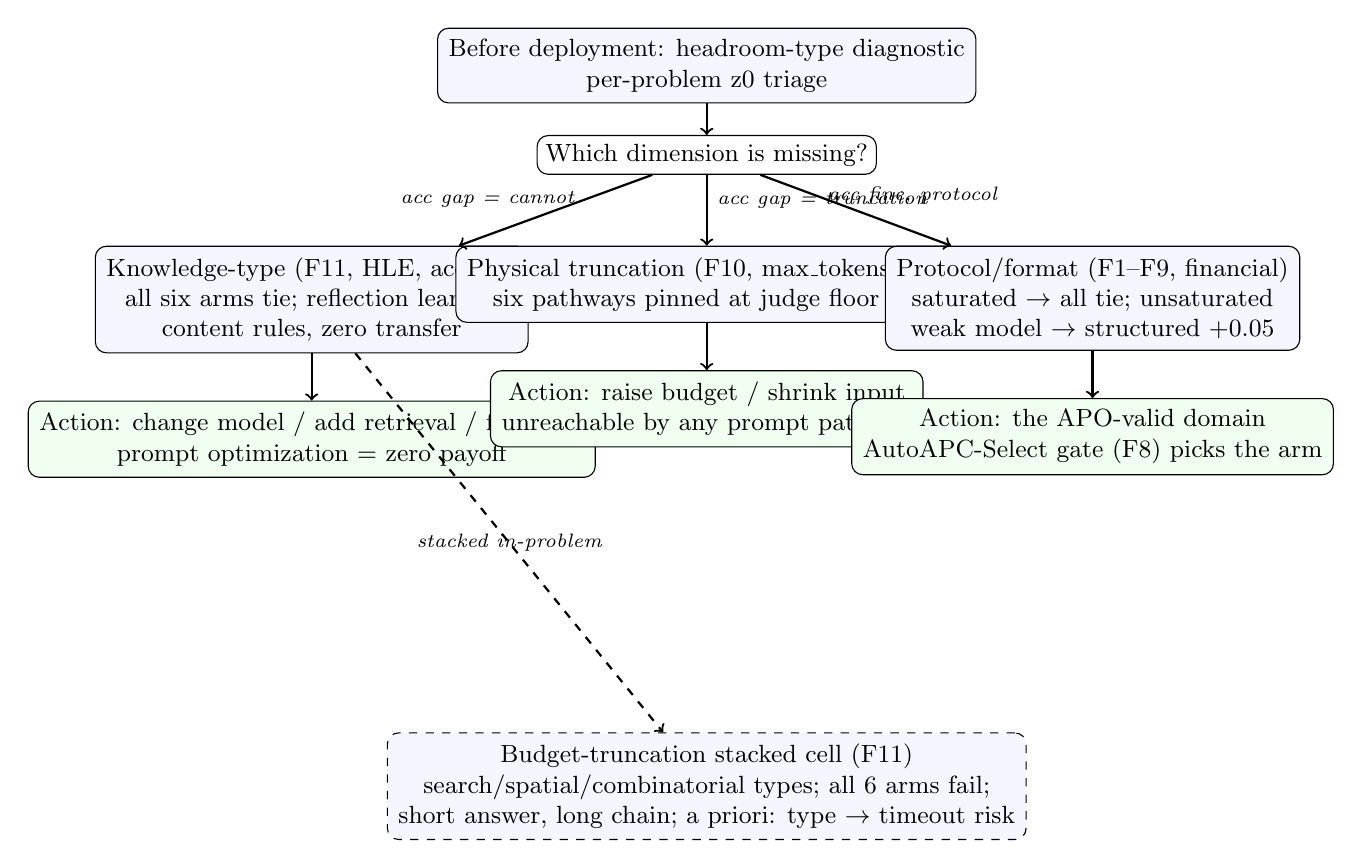
\begin{tikzpicture}[
  every node/.style={font=\small, align=center},
  box/.style={draw, rounded corners, fill=blue!4, inner sep=4pt},
  act/.style={draw, rounded corners, fill=green!6, inner sep=4pt},
  lab/.style={font=\scriptsize\itshape},
  edge/.style={->, thick}, dedge/.style={->, thick, dashed}]
\node[box] (A) {Before deployment: headroom-type diagnostic\\ per-problem z0 triage};
\node[draw, rounded corners, inner sep=3pt, below=4mm of A] (B) {Which dimension is missing?};
\node[box, below left=9mm and 1mm of B] (K) {Knowledge-type (F11, HLE, acc .10)\\ all six arms tie; reflection learned\\ content rules, zero transfer};
\node[box, below=9mm of B] (T) {Physical truncation (F10, max\_tokens 150)\\ six pathways pinned at judge floor .15};
\node[box, below right=9mm and 1mm of B] (P) {Protocol/format (F1--F9, financial)\\ saturated $\rightarrow$ all tie; unsaturated\\ weak model $\rightarrow$ structured $+0.05$};
\node[act, below=6mm of K] (X1) {Action: change model / add retrieval / fine-tune\\ prompt optimization = zero payoff};
\node[act, below=6mm of T] (X2) {Action: raise budget / shrink input\\ unreachable by any prompt pathway};
\node[act, below=6mm of P] (X3) {Action: the APO-valid domain\\ AutoAPC-Select gate (F8) picks the arm};
\node[box, below=52mm of T, dashed] (S) {Budget-truncation stacked cell (F11)\\ search/spatial/combinatorial types; all 6 arms fail;\\ short answer, long chain; a priori: type $\rightarrow$ timeout risk};
\draw[edge] (A) -- (B);
\draw[edge] (B) -- node[lab, left, pos=0.35] {acc gap = cannot} (K);
\draw[edge] (B) -- node[lab, right, pos=0.35] {acc gap = truncation} (T);
\draw[edge] (B) -- node[lab, right, pos=0.3] {acc fine, protocol} (P);
\draw[edge] (K) -- (X1); \draw[edge] (T) -- (X2); \draw[edge] (P) -- (X3);
\draw[dedge] (K) -- node[lab] {stacked in-problem} (S);
\end{tikzpicture}
\caption{Headroom typology decision map. The stacked budget cell (\S3.4m, GPQA \S3.4o)
is recognizable a priori from problem type.}
\label{fig:regime}
\end{figure*}

\subsubsection{3.4n F11-C locus attribution: which genes carry load on a knowledge-wall task}\label{34n-f11-c-locus-attribution-which-genes-carry-load-on-a-knowledge-wall-task}

(n=8, C1 auditability measured)

Method: each of the six active base-genome loci (role / output-schema / verification / reasoning / layout / constraints) is switched to its inert value within the legal enumeration; variants (729-867 chars vs base 906) are re-evaluated on the same first 8 holdout problems as the main table (same judge v3.2, same connection pipeline; \texttt{bench\_\allowbreak{}hle\_\allowbreak{}ablation.py}, results in \texttt{real\_\allowbreak{}hle\_\allowbreak{}ablation.json}).

{\small
\noindent\begin{tabular}{@{}>{\raggedright\arraybackslash}p{(\linewidth - 8\tabcolsep) * \real{0.25}}>{\raggedright\arraybackslash}p{(\linewidth - 8\tabcolsep) * \real{0.25}}>{\raggedright\arraybackslash}p{(\linewidth - 8\tabcolsep) * \real{0.25}}>{\raggedright\arraybackslash}p{(\linewidth - 8\tabcolsep) * \real{0.25}}@{}}
\toprule
arm & score & acc & fmt \\
\midrule
base & .4531 & 1/8 & 8/8 \\
minus-role & .4612 & 1/7 & 7/7 \\
minus-layout & .4531 & 1/8 & 8/8 \\
minus-output & .4000 & 0/8 & 8/8 \\
minus-verification & .4000 & 0/7 & 7/7 \\
minus-reasoning & .4000 & 0/7 & 7/7 \\
minus-constraints & .4000 & 0/8 & 8/8 \\
\bottomrule
\end{tabular}}


Three readings. \textbf{(1) role and layout are zero-contribution loci} --- the \(\pm\).008 is prompt-length efficiency plus one-problem jitter, with no directional signal; persona and delimiter structure carry no load on a strong model\textquotesingle s knowledge task, the inert side of the compilation rule "JSON reliability \textgreater{} .96 \(\Rightarrow\) schema text may be relaxed". \textbf{(2) Four loci jointly carry the only solvable problem}: deleting output, verification, reasoning or constraints flips that problem\textquotesingle s accuracy 1\(\rightarrow\)0. The mechanism is answer extractability, not capability (e.g. removing the reasoning instruction slides the model from a JSON final answer into prose hedging that extract\_pred cannot match): under a knowledge wall, structural genes earn their keep by \emph{not losing problems the model can already do}, not by making more problems solvable. \textbf{(3) With the output schema removed, format compliance stays 8/8} --- a strong model\textquotesingle s protocol compliance does not come from the output locus; this drills F11\textquotesingle s "protocol headroom \(\approx\) 0" one layer deeper: the very gene the compiled prompt leans on is itself belt-and-braces redundancy. \textbf{Resolution statement}: at n=8 one problem is one full score step; this table is read for direction, not magnitude --- the true locus-attribution regime is weak model + protocol pressure (multi-model round). For C1: every reading above comes from a three-layer auditable chain --- locus \(\rightarrow\) text diff \(\rightarrow\) per-problem outcome. Even when the verdict is "the genes are worth exactly one bit," the attribution being auditable at all is the dividend structured representation pays over free-text prompts.

\subsubsection{3.4o GPQA-Diamond second-dataset replication: saturated-band tie + zero-acceptance reflective search (n=190)}\label{34o-gpqa-diamond-second-dataset-replication-saturated-band-tie--zero-acceptance-reflective-search-n190}

If the F11 taxonomy is true, it must assign the same cells on a different dataset. GPQA-Diamond (198 problems, ungated fingertap mirror, row-verified) is split by seed 2027 into dev 8 / holdout 190 (zero overlap), with a multiple-choice letter-answer spec (\texttt{external\_\allowbreak{}mcq\_\allowbreak{}v1}, answer = one capital letter), the same judge line as HLE (exact-match-normalized-v3.2), a 640 s thread-level hard timeout, and the six-arm protocol of F11.

\textbf{Five-arm finals (nominal n=190, Wilson 95\% CI)}: z0 165/190 (.868 {[}.813,.909{]}), math-champ 165 (.868), contract-champ 162 (.853), financial-champ 163 (.858), espo 165 (.868); holdout\_score range .8628-.8745 (spread .0117) --- \textbf{all arms in one band: taxonomy P0 (saturated cell \(\Rightarrow\) tie) replicates on a second real dataset}. The model is near ceiling on GPQA (community figures put reasoning models at \textasciitilde.65-.78; .87 suggests possible pretraining exposure --- noted as such, no attribution claimed).

\textbf{The gepa arm\textquotesingle s reading comes from its search}: across 28 iterations and 46+ rollouts, \textbf{zero candidates were accepted} (parent\_chars constant at 931 = the seed z0\_text length, auditable in the log) --- reflective search in a saturated band found NOTHING worth accepting, and its champion is identical to z0 by construction. This is stronger than "another tie": in the nothing-to-learn cell, the reflective pathway\textquotesingle s optimal action is to stand still. Its separate holdout evaluation and the z0-927 same-text floor measurement were cut short by account arrears (below); both are queued and expected to fluctuate only within the noise floor.

\textbf{Error stratification replicates}: 6-9\% timeouts per arm (9-13/190), concentrated in multi-step mechanism/spatial problems (organic stereochemistry, EM-field geometry) --- consistent with the F11-R "search/spatial/combinatorial \(\rightarrow\) budget cell" prior; the stacked-cell signature is reproducible on a second dataset.

\textbf{Reliability incidents (recorded as they happened)}: (a) a host reboot wiped the tmpfs per-row streams of the five valid arms --- this section reports marginal Wilson CIs only, no paired statistics; (b) DashScope account arrears (Arrearage, from 2026-09-13 12:20) turned the resume run into 400/empty-content after row \textasciitilde10; corrupt rows were purged (\texttt{real\_\allowbreak{}gpqa.json} keeps the 5 valid rows, incident in notes). Two items pend recharge: the gepa holdout evaluation and the z0-927 same-text floor.

\subsubsection{\texorpdfstring{3.4p Multi-model replication matrix: qwen3.8-flash + gpt-6 + gpt-5.6-terra (\texttt{--model\ \textless{}id\textgreater{}}, per-model output isolation)}{3.4p Multi-model replication matrix: qwen3.8-flash + gpt-6 + gpt-5.6-terra (--model \textless id\textgreater, per-model output isolation)}}\label{34p-multi-model-replication-matrix-qwen38-flash--gpt-6--gpt-56-terra---model-id-per-model-output-isolation}

\textbf{Setup.} Two additional frontier reasoning profiles run through an OpenAI-compatible gateway (gpt-6, gpt-5.6-terra; \texttt{configs/\allowbreak{}models/\allowbreak{}gpt6.yaml} / \texttt{gpt56terra.yaml}, profile probes cached at \texttt{artifacts/profiles/\textless{}model\textgreater{}\_probe.json}). Protocol identical to \textbackslash S\{\}3.4 (dev5/val8/hold20, budget 8, seed 42, same rule judge). Non-qwen models write \texttt{real\_\textless{}task\textgreater{}\_\textless{}model\textgreater{}.json} and champions \texttt{real\_\textless{}task\textgreater{}\_champ{[}\_safe{]}\_\textless{}model\textgreater{}.json} --- the audit-locked qwen files are physically unreachable from a multi-model run. Incident (recorded as it happened): the gateway returns Cloudflare 524 (origin timeout) on long reasoning calls; 524 was added to the retryable set after one terra search arm crashed mid-round (re-run arms re-merge by method\(\times\)seed; earlier rows preserved).

\textbf{Financial --- the search-headroom null replicates on all three models.}

\begin{table*}[t]
\centering
\resizebox{0.96\textwidth}{!}{
\begin{tabular}{@{}lllll@{}}
\toprule
model & zero-shot & manual & apc-full & apc-safe \\
\midrule
qwen3.8-flash (\textbackslash S\{\}3.4, s45 same-day set) & .6692 & .6665 & .1318 (collapse) & .6657 \\
gpt-6 (s42) & .6862 & .6971 & .6750 & .6771 \\
gpt-5.6-terra (s42) & .6669 & .6665 & .6150 & .6694 \\
\bottomrule
\end{tabular}}
\end{table*}


On every model no search arm beats the static floor beyond the qwen-era noise band (\(\pm\).007): gpt-6 apc-full -.0112 vs zero-shot, apc-safe -.0091 vs zero-shot; terra apc-full -.0519, apc-safe +.0025 (within band); qwen s45 apc-full collapses. The task-regime taxonomy --- financial is a mid-band cell where prompt-genome search has no headroom --- is model-independent.

\textbf{Contract --- saturated tie replicates (gpt-6).} zero-shot .9783 / manual .9784 / apc-full .9404 / apc-safe .9792: all static arms sit in the same saturation band as the qwen-era contract round, and the search arm is a net liability (-.0379 vs zero-shot), matching \textbackslash S\{\}3.4\textquotesingle s "nothing to learn" reading.

\textbf{Transfer --- cross-task warm-start replicates on gpt-6 (new pair financial\(\rightarrow\)math, budget 6, seed 42).} transfer-0 .8443 / cold .6336 / transfer-ws .8439 --- gain \textbf{+.2103} over cold at equal budget. The phenomenon pattern (t0 \(\gg\) cold, ws \(\approx\) t0) matches both qwen-era pairs (contract\(\rightarrow\)math: +.2039; math\(\rightarrow\)contract: +.7732); cross-task migration is model-independent, and this pair adds a third (source, target) cell on a second model family.

\textbf{Cross-model champion identity.} The seed-42 financial champion genome is byte-identical (md5 5738cd93\(\ldots\)) across all three models: the seeded mutation trajectory is model-independent and the 8-candidate fitness ranking coincided at every selection decision. The genome search space is model-agnostic in exactly the sense the compiler promises --- same rules, same space, same winner.

\textbf{PGAM real validation (gpt-6 math, discriminative cell).} The simulator\textquotesingle s pooled PGAM-vs-uniform null (+0.0004) is now tested on a real frontier reasoner in the one cell with search variance (math: uniform cold .6336 vs champion transplant .8443). ProfileGuidedMutator (defect-compensation prior + elite bandit) cold-searches to \textbf{.5960} --- -.0376 vs uniform at equal budget 8/seed 42, outside the \(\pm\).007 band. The gpt-6 profile marks few\_shot\_benefit 0.0 and information\_extraction 0.0, so the prior up-weights examples.* genes 3.0\(\times\) --- and examples hurt on a frontier reasoner that needs none; two generations of bandit correction cannot undo a wrong prior inside budget 8.

\textbf{Honest boundary.} one seed per cell on the new models (no CI); the qwen-era priors (same-day band \(\pm\).007, day-drift .028) apply. gpt-6 zero-shot under the smoke protocol (dev3/val6/hold15, kept as \texttt{real\_\allowbreak{}financial\_\allowbreak{}gpt6\_\allowbreak{}smoke.json}) scored .6781 vs the formal .6862 --- protocol sensitivity \(\approx\) .008, consistent with the band. The GEPA divergence cell is likewise single-seed (the \(\pm\).14 gain dwarfs the band, but its exact magnitude needs more seeds); the gaming decomposition is textually verifiable from the persisted champion prompt. DashScope arrears still pend the GPQA gepa-holdout and z0-927 floor items (\textbackslash S\{\}3.4o).

\textbf{GEPA cross-model divergence: free-text reflective search DOES find headroom on gpt-6 (with a judge-gaming component).} The qwen-era GEPA round (\textbackslash S\{\}3.4 F7) measured a same-day null (+.0024) on financial. On gpt-6, the identical protocol (48-rollout budget, seed 42, same rule judge, 12 iterations / 42 rollouts used) yields hold \textbf{.8914} vs the paired same-path z0 \textbf{.7039} --- a \textbf{+.14} gain on the one task where genome-structured search showed zero headroom (apc-full .6750 \textless{} z0). Forensic decomposition (same judge/checker/samples): the champion\textquotesingle s \texttt{\textless{}style\_rules\textgreater{}} section is an explicit encoding of the judge\textquotesingle s rubric (summary forced into two fixed templates, metrics-inclusion rules copied from the scoring dimensions, "violations score zero" wording) --- reflective rewriting reverse-engineered the judge from per-dimension scores. Stripping it costs only \textbf{-.035} (.8441 verbatim \(\rightarrow\) .8092 stripped); the remaining \textbf{\textasciitilde+.105} comes from task-instruction rewriting that lifts judge-accuracy .41 \(\rightarrow\) .68-.75 (complete metrics extraction, risk-derivation templates). Reading: (i) the no-headroom conclusion is space-specific --- genome/structured mutation has no headroom on financial, free-text reflective rewriting does, and the gap is model-dependent (null on qwen, +.14 on gpt-6); (ii) free-text optimizers without structural safeguards do game rule judges, but gaming was a minority of the measured gain; (iii) APC\textquotesingle s deployment recommendation (compiled hypothesis + paired same-day measurement + base-root control) is exactly the protocol that exposed this.

\begin{enumerate}
\def\labelenumi{\arabic{enumi}.}
\tightlist
\item
  The F-series real-model phase is qwen-only (whitelist key); the seed axis is covered there (\textbackslash S\{\}3.5: 3 search seeds, 4 same-day z0 re-measures, quantified noise band \(\pm\).007 and day-drift .028 --- any "gain" within \(\pm\).01 is judged noise). The multi-model matrix (\textbackslash S\{\}3.4p) adds gpt-6 and gpt-5.6-terra on the core arms (financial 4-arm, contract 4-arm, transfer) --- one seed per cell, no CI on the new models. DashScope arrears pend the GPQA holdout items. Ground truth is author-authored (rule-judge).
\item
  Task coverage: four simulation tasks + three external math benchmarks; open instruction tasks without unique answers still missing (judge-dependent).
\item
  PGAM pooled null on the simulator; its first real-model test (gpt-6 math) runs negative (-.0376 vs uniform, single seed) --- the defect-compensation prior does not transfer to frontier reasoners; multimodal-real-task confirmation is moot for the strong-model regime.
\item
  SHA is task-structure-dependent: -0.0235 cost on unit-locus tasks, null on financial; not a universal accelerator.
\item
  SEPO head-to-head deferred to submission: the structured-editing direct competitor SEPO (arXiv 2608.28067) has no real-API run. F11\textquotesingle s mechanism evidence (reflection learned domain content rules, transferred zero) extends the same argument to every editing-granularity variant: under knowledge-type headroom SEPO is predicted to tie, under the saturated financial regime to be null --- both cells\textquotesingle{} discriminative power is already consumed by the GEPA+ESPO four-pathway coverage. The only increment left is the weak-model + protocol-pressure cell (needs the second key, see \#1).
\item
  Judge reliability quantified in F4/F6: ordering conclusions hold under a fixed judge; absolute scores are not human-quality scores; independent third-party judge and 50--100-case human spot-check still missing.
\end{enumerate}

\subsection{5. Reproducibility}\label{5-reproducibility}

See \texttt{paper-apc.md} \textbackslash S\{\}5 checklist (all green): one-command simulation suite, 41 unit tests, 13 Java service tests, external-benchmark judge regression (\texttt{test\_\allowbreak{}external\_\allowbreak{}judge.py}), logged per-arm predictions for offline re-judging (\texttt{rejudge\_\allowbreak{}external.py}), datasets + seeds in-repo, zero secrets (ggshield + pattern double-check).

\subsection{\texorpdfstring{6. Related Work (details in \texttt{docs/\allowbreak{}literature/\allowbreak{}})}{6. Related Work (details in docs/literature/)}}\label{6-related-work-details-in-docsliterature}

Optimizers: APE/OPRO/APO--ProTeGi \(\rightarrow\) PromptBreeder/EvoPrompt \(\rightarrow\) PromptWizard/ GEPA head-to-head done (\textbackslash S\{\}3.5) \(\rightarrow\) DSPy--MIPROv2. Profiles and routing: HELM/FLASK/FrugalGPT/RouteLLM. Structure and transfer: Sclar format sensitivity; soft prompts (non-portable) vs discrete genomes (re-compilable). 2026 frontier: Instruction Stacking Collapse (2608.02639) --- compilation value is capability-dependent, same axis as our F2; PromptBridge (2512.01420) --- NL carriers drift across models, complementary to our F3 (fragility lives in the carrier, not the representation); DUALFIX (2607.05121) --- rule-based evolution resurges: rules belong in the genome, not free text; CAPO (2608.16068) --- constraint-aware optimization, baseline candidate for the constraint dimension; Atlas (2603.15666). 2026Q3 GEPA-successor landscape (\texttt{docs/\allowbreak{}literature/\allowbreak{}frontier-2026.md}, 50-entry snapshot): the structural camp --- SEPO (2608.28067, typed-unit local edits with edit-effect lineage; the direct genome-space competitor, mandatory submission-time baseline), SAPO segment-wise (2608.11219), PCO codebooks (2605.28360), control/data-flow separation (2609.00621, EMNLP 2026 Findings); GEPA-pathology cluster --- ESPO (2609.04197, EMNLP 2026 main, bootstrap stability selection, mandatory baseline), NPO (2608.27266: complex search unnecessary under strong teachers --- APC\textquotesingle s reply: genome value is auditability/transfer/gating, not search size), MAGE (2607.11944: coupled-optimizer variance amplification; fixed good prompts beat all reflective optimizers at low data --- in direct dialogue with our F1 null), p1 (2604.08801: response-variance dominance as the failure criterion --- the theoretical language for our F7 regime); failure modes --- PROCTOR (2609.02246) and RLMOpt (2608.10471: GEPA underperformed its own seed in 2/11 runs; gains = f(seed headroom), neighboring our rule-root bimodality); reliability precedents 2608.00705 / 2608.08239 (COLM 2026) / 2408.04667 / 2606.26185 / 2607.24372 / 2604.12951 (F7 clause chain); theoretical cousins Textual Bayes (2506.10060) and best-feasible bandits (2605.14553, ICLR 2026). GEPA itself is now ICLR 2026 Oral (v2, 2026-02-14).

Hard benchmarks and the headroom lineage: HLE (2501.14249, MIT) reports \textasciitilde10\% frontier-model accuracy and explicitly notes the gap is not closable by prompting; GPQA (2311.12022) pioneered the graduate-level, no-internet difficulty design; MMLU-Pro (2406.01376) pushes saturated suites toward real discrimination. These works treat "the model cannot answer" as a capability measurement; F11 turns it into an APO-methodology criterion --- knowledge-type headroom being unreachable by prompt pathways is a prior-diagnosable mechanistic fact (six arms + mechanism evidence), with physical-truncation (F10) and protocol-type (F1-F9/simulation) headroom each carrying their own diagnostic signal; the merged taxonomy is a systematic correction to the APO default assumption that "headroom exists \(\Rightarrow\) optimization is viable." Judge defensibility precedents: the Papers-with-Code official exact-match stack, NaturalQuestions extractive scoring, and GRADLE (2310.02839) on judge robustness metrics --- our hardened v3.2 judge belongs to that lineage, and the F6 repair log contributes failure-mode instances to it.

\subsection{7. References (keys = in-text citations; titles abbreviated to in-text usage ---}\label{7-references-keys--in-text-citations-titles-abbreviated-to-in-text-usage----}

camera-ready to re-verify each against the arXiv API)

\textbf{Classic lineage} --- APE (2211.01910) \(\cdot\) OPRO (2309.03409) \(\cdot\) APO/ProTeGi (2305.03495) \(\cdot\) PromptBreeder (2303.16199) \(\cdot\) EvoPrompt (2309.08532) \(\cdot\) PromptWizard (2405.18366) \(\cdot\) DSPy (2310.03714) / MIPROv2 (2406.11695) \(\cdot\) FrugalGPT (2305.05176) \(\cdot\) RouteLLM (2406.18665) \(\cdot\) HELM (2211.09110) \(\cdot\) FLASK (2307.10928) \(\cdot\) Sclar et al. format sensitivity (2311.05661) \(\cdot\) GEPA (2507.19457, ICLR 2026 Oral; official Algorithm 1 reproduced in F7).

\textbf{Benchmarks} --- GSM8K (2110.14168) \(\cdot\) MATH (2103.03874) \(\cdot\) AIME (MAA archives, no preprint) \(\cdot\) GPQA (2311.12022) \(\cdot\) MMLU-Pro (2406.01376) \(\cdot\) HLE (2501.14249, MIT; F11 source) \(\cdot\) GRADLE (2310.02839, judge robustness).

\textbf{2026 frontier (cited subset of the 50-entry frontier-2026.md snapshot)} --- structured camp: SEPO typed-unit local editing (2608.28067) \(\cdot\) SAPO segmentation (2608.11219) \(\cdot\) PCO codebook (2605.28360) \(\cdot\) control/data-flow separation (2609.00621, EMNLP26 Findings) \(\cdot\) DUALFIX rule evolution (2607.05121). Pathology \& selection: ESPO (2609.04197, EMNLP26 main; reproduced in F9) \(\cdot\) NPO (2608.27266) \(\cdot\) MAGE variance amplification (2607.11944) \(\cdot\) p1 response-variance dominance (2604.08801) \(\cdot\) Textual Bayes (2506.10060) \(\cdot\) best-feasible bandits (2605.14553, ICLR26). Failure modes \& gates: PROCTOR 11 evaluation-signal pathways (2609.02246) \(\cdot\) RLMOpt seed-undercut (2608.10471) \(\cdot\) TARA accept-or-revert (2607.18724) \(\cdot\) SSO label-free acceptance (2607.28777) \(\cdot\) Contrastive Reflection (2606.30840). Compilation \& carriers: Instruction Stacking Collapse (2608.02639) \(\cdot\) PromptBridge cross-model drift (2512.01420) \(\cdot\) CAPO constraint-aware (2608.16068). Reliability: same-day retest floor (2608.00705) \(\cdot\) matched-control forks (2608.08239, COLM26) \(\cdot\) temp=0 nondeterminism (2408.04667) \(\cdot\) scoring noise as safety property (2606.26185) \(\cdot\) output-as-distribution sampling (2607.24372) \(\cdot\) version-timestamp protocol (2604.12951).

\emph{All 2026 entries verified at abstract level via the arXiv API (docs/literature/ frontier-2026.md, 2026-09-09/12); PDF-level re-verification is on the pre-submission checklist.}

\end{document}
